\chapter{Analysis}


With this data, we were able to further investigate accuracy and general glucose analysis. As previously mentioned, capillary blood glucose is considered the clinical gold standard for most treatment. While our app provided a quick, easily accessible way to read the sensor, the returned values were not a perfect fit for either simultaneous BGM readings or the Freestyle Libre reader, which processes the raw values for greater accuracy. We hoped that, with further analysis, we would be able to improve on this accuracy. 

The reverse engineering mentioned above provided four datasets in total. The blood glucose readings individually added from fingerpricks, the raw sensor values from our app, the manual readings reported by the reader, and the extracted dataset contained in the reader memory.

\section{Data Comparison}
The processed data\footnote{referring to the 15-minute data collected from the reader, and raw data likewise refers to data directly extracted from the sensor.} - provided by \$history - is distinctly different from the raw data, as shown by Figure~\ref{fig:graph3}. It is also (excluding the separate manual dataset) evenly spaced 15 minutes apart. This suggests that the processed data is a transformed version of the 15 minute raw datasets. The data displayed on demand with each scan is intended to estimate the current blood glucose level - let's call this read-time data (alternatively manual data, since it is affected by the manual scanning of the sensor). Interestingly, these manually pulled values heavily deviate from the other processed data, as seen in Figure~\ref{fig:graph4}. 

The most obvious reason for this would be an attempt to make up for the time lag between interstitial fluid and blood glucose. On the other hand, this is probably taken into account with all the processed data, which Figure~\ref{fig:graph3} would appear to support. Another option is that the difference is due to the calculation method. The majority of the processed data may be calculated solely off the sensor-provided 15 minute data, even if higher definition data is available, while the read-time value incorporates the 30 minutes of dense data into the calculation. The latter theory suggests that the read-time values should be more accurate than the rest of the processed data.

\begin{figure}[ht]
\centering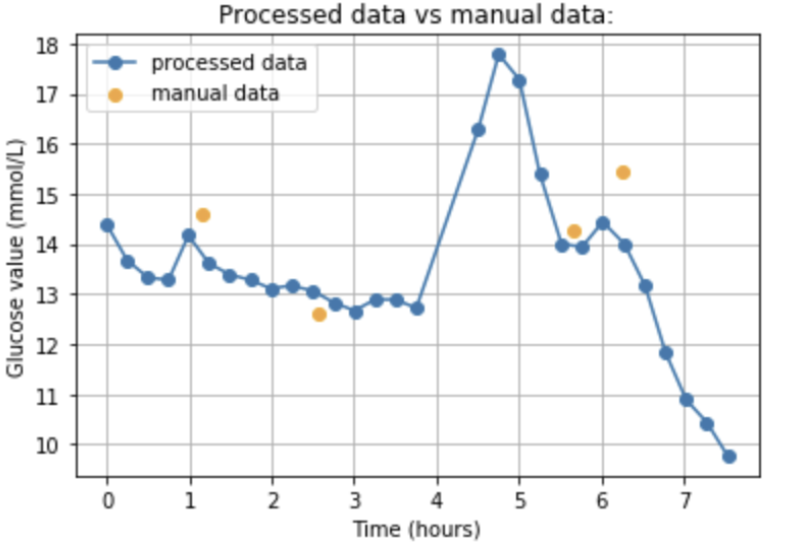
\includegraphics[width=0.7\linewidth]{images/graph4.png}
\caption{Graph of read-time reader data.}
\label{fig:graph4}
\end{figure}

We lacked the data to do a proper accuracy evaluation, and many papers have already done so. 

When it comes to accuracy, the Freestyle Libre consistently underperforms BGMs, but not to a debilitating extent. However, in some studies it has been found to fall short of common specifications - Fokket et al. found only 85.5\% of results fell within Zone A of the Clarke Error Grid, which has a generally accepted requirement of 95\%. Over use, we found that the average difference between almost simultaneous BGM and reader readouts was comparable to the average difference between two semi-simultaneous readings taken with the same BGM, as shown in Figure~\ref{fig:cgmvsbgm}. The exception to this were three troubling outliers, where the Libre read significantly under (5-8mmol/L) the BGM ground truth. This is a noticeable trend - the CGM routinely underestimates the BGM glucose reading, especially during hypoglycemia. 

\begin{figure}[ht]
\centering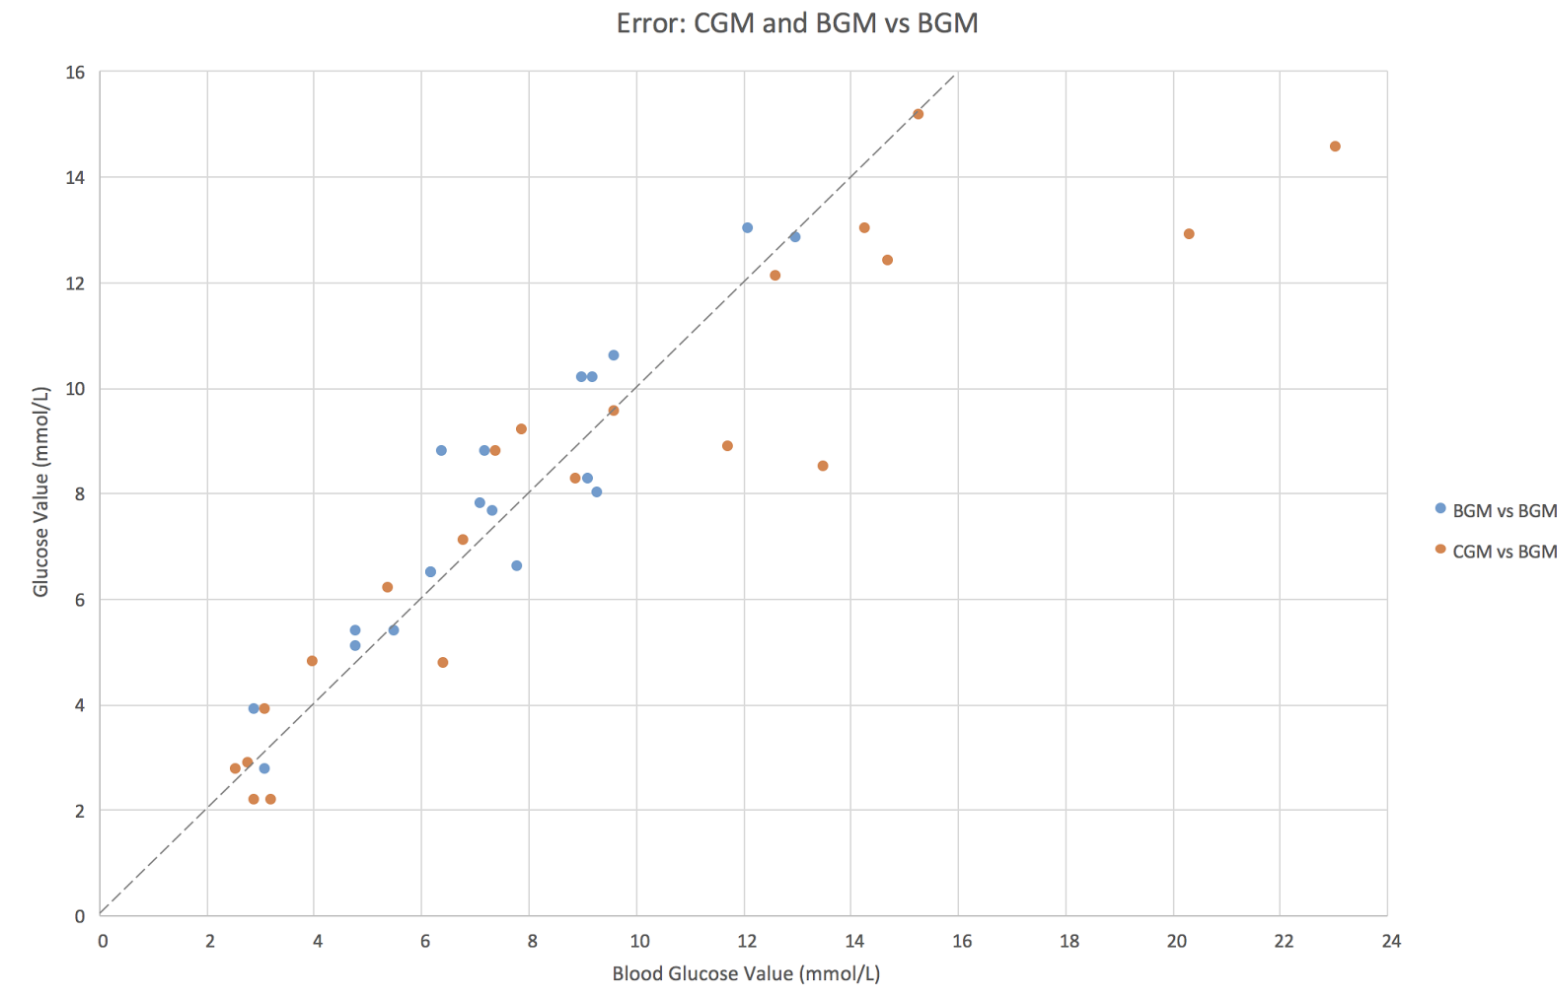
\includegraphics[width=1\linewidth]{images/cgmvsbgm.png}
\caption{Comparison of the correlation between the Freestyle Libre and a BGM measurement with a simultaneous BGM ground truth.}
\label{fig:cgmvsbgm}
\end{figure}

Figure~\ref{fig:diffbell} shows the distribution of the differences between the BGM reading and another simultaneous reading from either the same BGM or the CGM. The CGM clearly does not perform as well as the BGM, although this is significantly improved if the outliers are removed from consideration. Given the 15 minute delay due to intravenous fluid, this is understandable. If anything, it’s surprising how much variation there was between two semi-simultaneous readings on the exact same meter.

\begin{figure}[ht]
\centering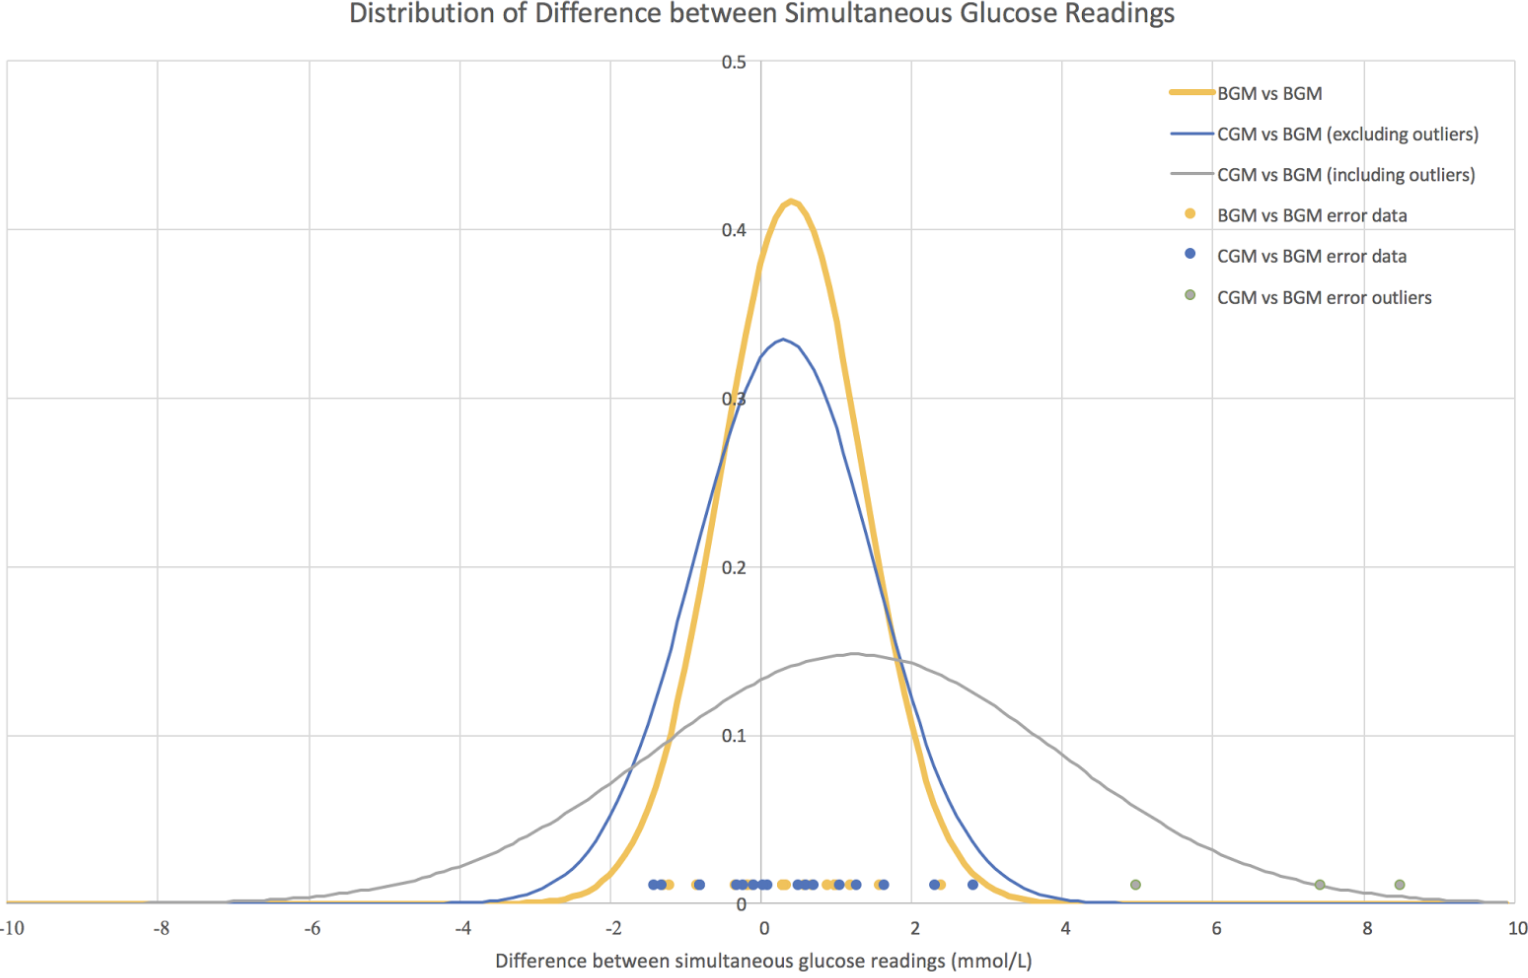
\includegraphics[width=1.0\linewidth]{images/diffbell.png}
\caption{Gaussian distributions of the difference between simultaneous BGM readings and simultaneous BGM and Libre readings.}
\label{fig:diffbell}
\end{figure}

These findings held true when comparing the limited blood glucose (fingerprick \textit{ground truth}) readings against the available time data, as in Figure~\ref{fig:graph0}. The Freestyle Libre was usually reasonably accurate to the BGM measurement, even when glucose was changing quickly. The processed reader values were more accurate than the raw values, as expected. Where applicable, the manual readings were usually a bit closer still. As previously mentioned, it sometimes wildly underestimated particularly high blood glucose reading, so it is possible that these points of apparent mismatch  may be user error, with the BGM reading incorrectly high due to sugar on the fingers or the needle, for instance. Of course, there isn’t enough data to form a true conclusion either way.


\begin{figure}[ht]
\centering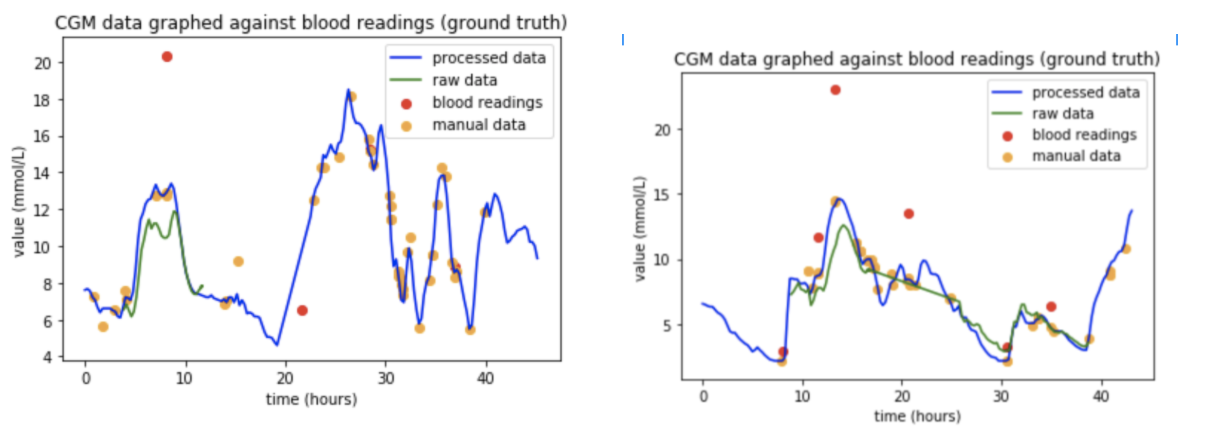
\includegraphics[width=1.0\linewidth]{images/graph0.png}
\caption{Multiple graphs comparing blood glucose data with CGM.}
\label{fig:graph0}
\end{figure}

\section{Prediction}
One of the major additional features that a CGM brings is an element of prediction through data analysis. Improving accuracy of this is very helpful. As previously explained, Freestyle Libre communicates predictions with arrows (see Figure~\ref{fig:arrows}), which translate to the direction glucose is currently trending in mmol/L per minute. First, the accuracy of this needed to be evaluated. The majority of the data we had came in fifteen minute intervals, but it was simple arithmetic to translate the arrow meaning into mmol/L per 15 minute. Matching the time of each manual scan (and hence arrow) to the closest 15 minute change in processed data, an acceptable ground truth, allowed me to get the accuracy of the Freestyle Libre arrows. Depending on the time frame, this varied around 63\% +-5. This seemed fairly low, so effort was made to improve on it using both least squares linear regression and neural networks.

\subsection{Linear Regression}
The initial attempt at linear regression was at seeing whether curve fitting data could be extended to predict future values. As Figure~\ref{fig:graph6} shows, this was predictably unsuccessful. Extending the curve quickly got out of hand, with even the first values being very poorly fit. 

\begin{figure}[H]
\centering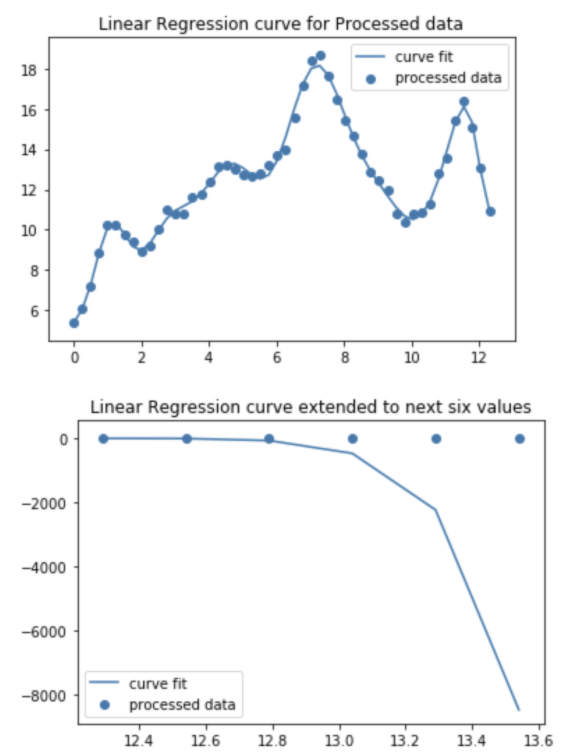
\includegraphics[width=1.0\linewidth]{images/graph6.png}
\caption{Linear Regression results.}
\label{fig:graph6}
\end{figure}

Next, I tried predicting the change in value based on the past 20 datapoints. This initially seemed far more successful than the prior attempt, and even than the reader itself, as shown in Figure~\ref{fig:graph6_5}. The accuracy was taken from testing with separate data, not the training set. While there was some fluctuation depending on the training/test sets chosen, it was consistently above 70\%. Attempting to improve on this - to predict over an hour, to take derivative values as input, to add prior - made little improvement, or caused a backtrack. Nevertheless, it seemed pretty successful.

\begin{figure}[H]
\centering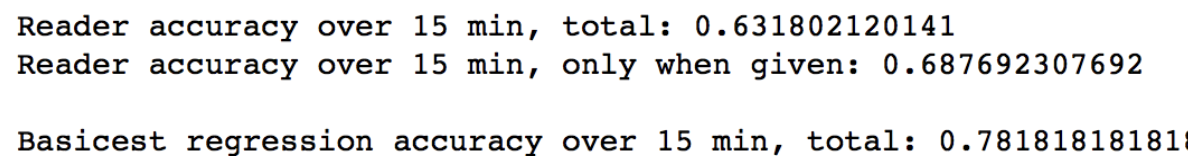
\includegraphics[width=1.0\linewidth]{images/graph6_5.png}
\caption{Linear Regression results on prediction.}
\label{fig:graph6_5}
\end{figure}

\subsection{Neural Networks}
The next attempt at improving on the prediction arrow was a basic neural network, which I expected to be quite successful. However, it would always immediately go to 78\% accuracy and refuse to move through epochs or re-runs, as in Figure~\ref{fig:graph7}. It fluctuated somewhat depending on the testing data, but it was generally settled. This behaviour seemed strange, so I looked further into it.

\begin{figure}[ht]
\centering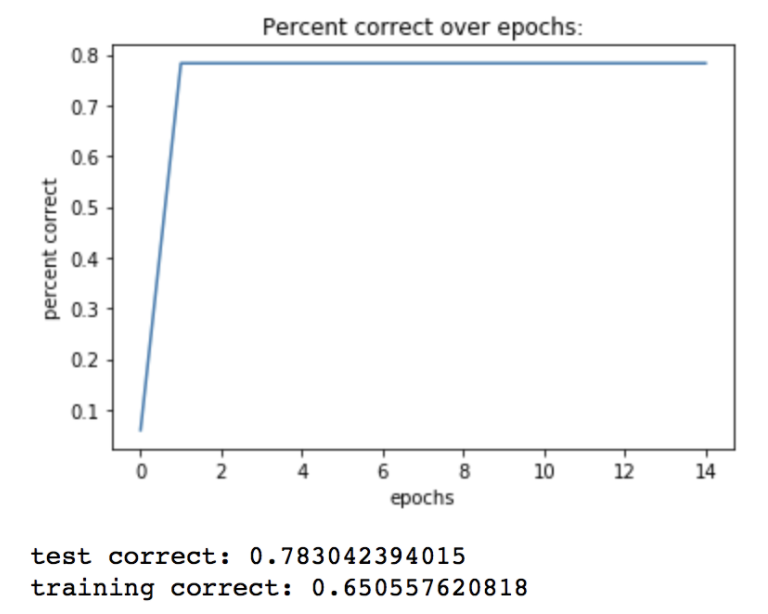
\includegraphics[width=1.0\linewidth]{images/graph7.png}
\caption{Training error against epoch for neural network.}
\label{fig:graph7}
\end{figure}

As it turned out, the problem was that the data was generally too easy to predict. Averaging $\frac{3}{4}$ of it was going straight. This meant the neural network was just persistently returning \textit{straight}, getting it right most of the time, and not changing. In fact, looking back at the linear regression, it suffered the same fault. As Figure~\ref{fig:graph8} shows, the ground truth for the change in value varied between -4 and 4, albeit heavily clustered around zero. The prediction, on the other hand, remains tightly between -1 and 1. This means it still captures most of the data accurately, but ignores two thirds of the possible range.

\begin{figure}[ht]
\centering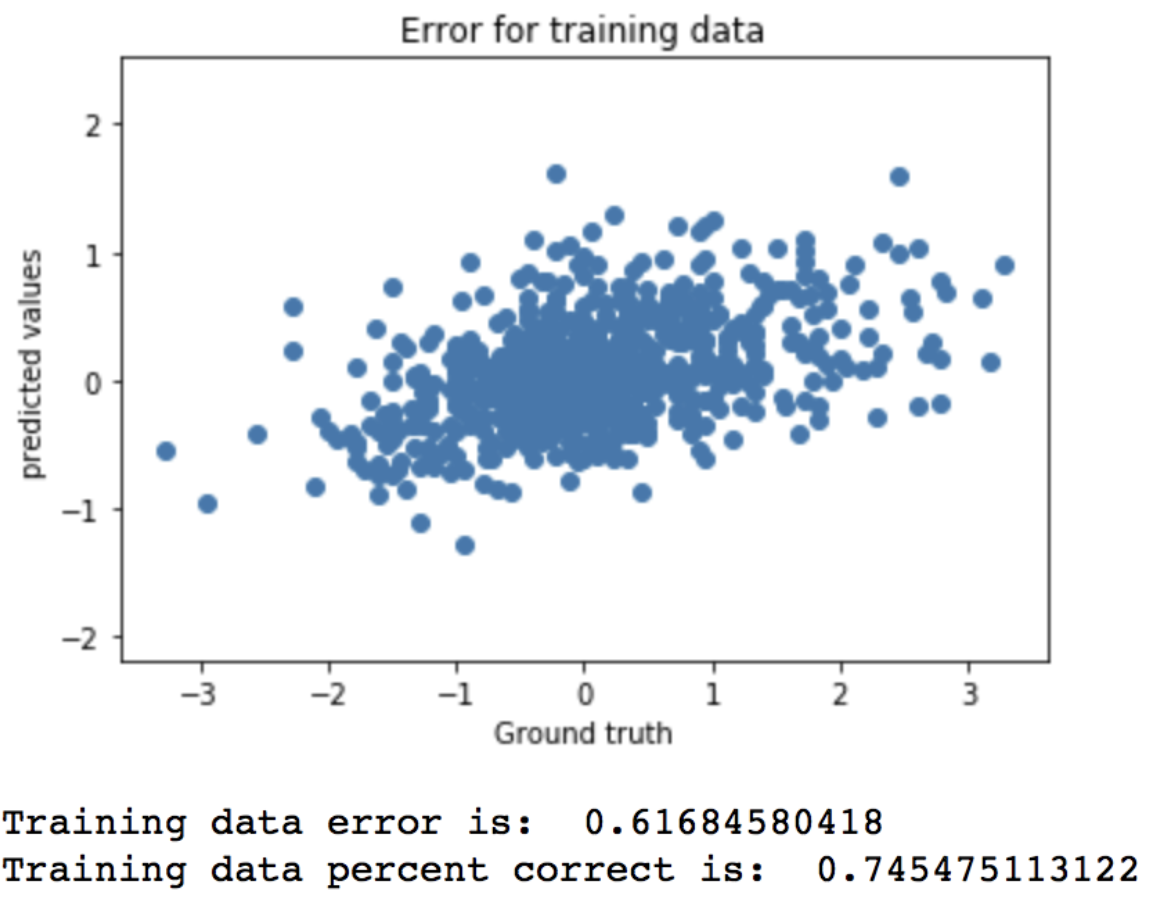
\includegraphics[width=1.0\linewidth]{images/graph8.png}
\caption{Correlation data for prediction.}
\label{fig:graph8}
\end{figure}

\subsection{Reader Prediction Arrow}
The reader’s glucose trend arrow had a poorer mathematical accuracy than either of my algorithms, while displaying the full range of directions instead of just straight. To better understand how this went, I broke down their correct and incorrect instances, as shown in Figure~\ref{fig:graph9}. This shows the distribution of the correct matches, the incorrect arrows, and the incorrectly represented ground truths across the trend directions; the distribution of the differences between a displayed arrow and the corresponding true direction, and a more detailed breakdown of the errors. These numbers tell us a few things.

\begin{figure}[H]
\centering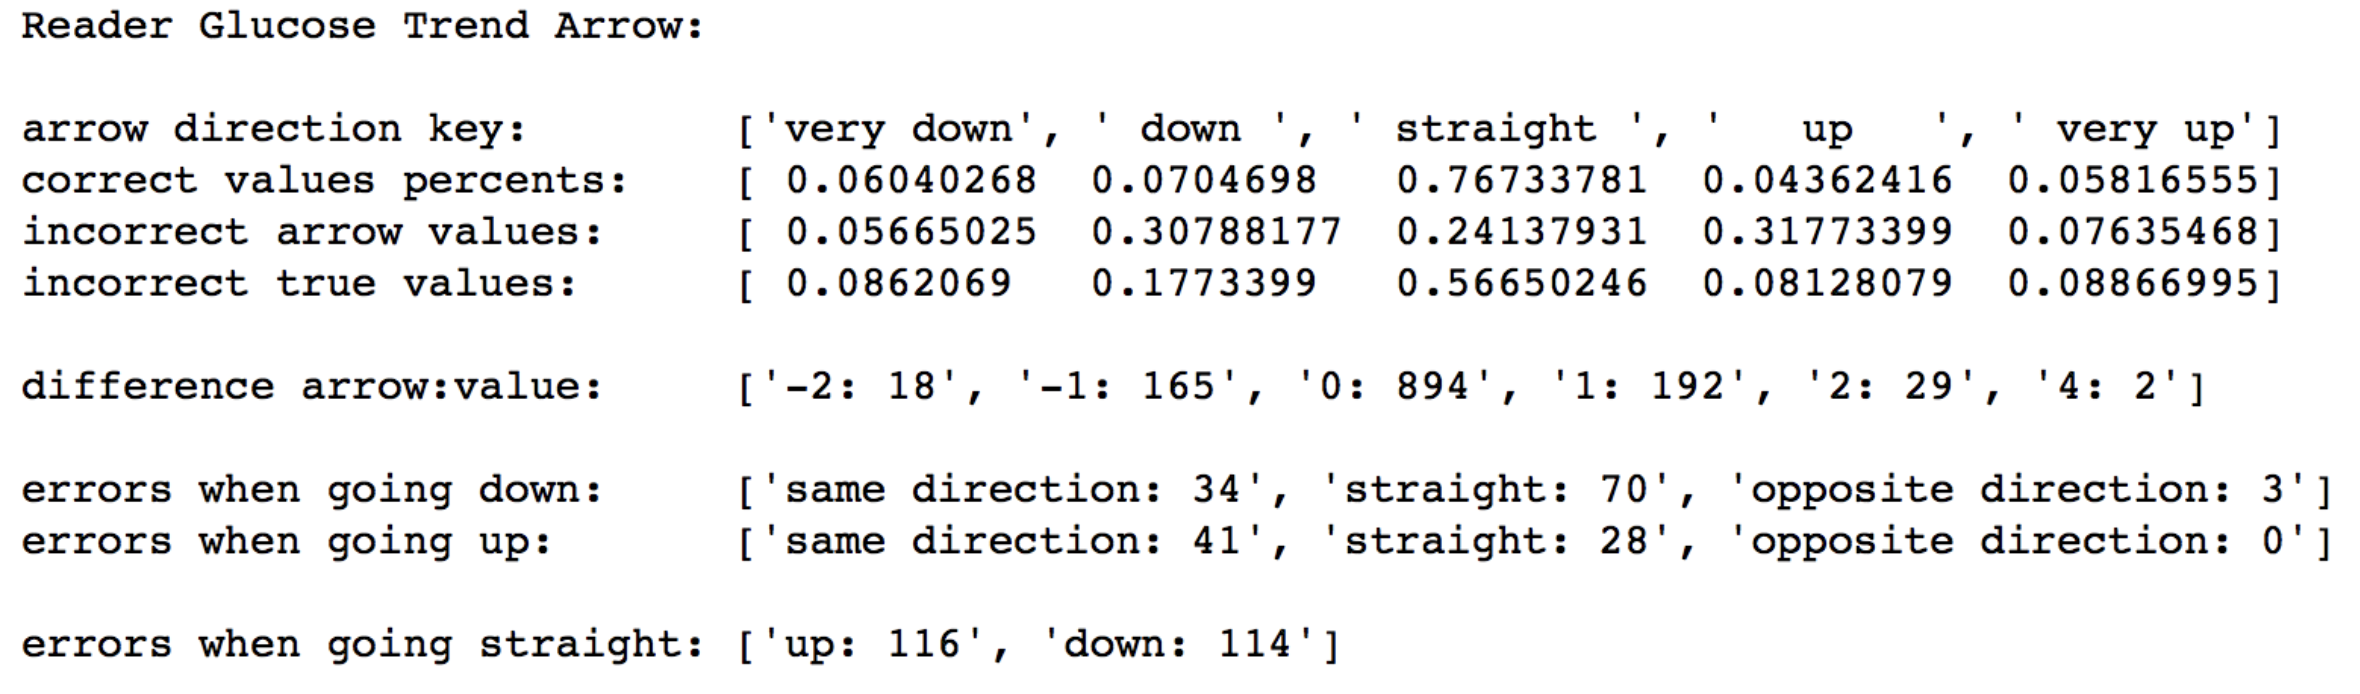
\includegraphics[width=1.0\linewidth]{images/graph9.png}
\caption{Trend arrow statistics.}
\label{fig:graph9}
\end{figure}

First, while the reader is often inaccurate, it’s rarely completely incorrect. Almost 93\% of the predictions is within one degree of the ground truth. Less than 2\% is further away than two degrees. On the other hand, that 2\% is an extreme enough difference to possibly cause harmful management decisions (eg: the difference between 4.2 going straight down, and going straight up). 

The reader exaggerates change. When the reader is correct, it displays a straight arrow 77\% of the time. When the reader is incorrect, it is much more likely to be signalling a change in glucose, only showing straight 24\% of the time. This suggests that the reader algorithm is more responsive to changes in blood glucose than steadiness, and is likely to over exaggerate change in blood glucose. This is in direct contrast to my attempts, which actively conformed everything to ‘straight’, so all the incorrect values were due to rapidly changing bloods being typed as ‘straight’ nonetheless.

On the other hand, the true gradient is more likely to be changing when the reader is incorrect. When the reader was incorrect, the gradient was changing 44\% of the time. This is almost twice the amount when the reader was correct, 23\%. The reader is more likely to read incorrectly on a quickly changing value. Some of this might be overestimating the rate of change, but the rest will be due to underestimating the change. This is in contrast to the early statistics, which suggested that the reader perpetually overestimated change.

With the incorrect readings, the distribution of the true gradient was slightly skewed down. The given arrow value was slightly skewed up. This suggests the reader is more likely to incorrectly predict a higher gradient.

Of the errors that occur while the true value is straight, the uncertainty is very equally distributed between over and underestimating. This suggests a lack of bias. Similarly, the reader has only pointed in completely the wrong direction once. 

When true trend is going down, 60\% of the reader’s incorrect predictions go straight. Only 30\% of the time will an incorrect arrow get the direction, at least, correct. In contrast, if the true trend is up, an incorrect prediction is 60\% likely to be in the right direction, just with the wrong severity. The suggests that the reader arrow exaggerates upwards trends and downplays downwards trends.

The reader’s glucose trend arrow has avoided the trap of only ever predicting straight, while maintaining decent accuracy ratings. It appears to do this by magnifying any change there is in the trend, often resulting in incorrectly predicting more change than there is. This could be due to technical issues preventing greater accuracy. On the other hand, it is most likely due to the arrow's purpose as a clinical treatment aid, not a mathematical instrument. Abbott's internal research may suggest that better treatment decisions are made when glucose rate of change is made more obvious.



\subsection{Clinical Analysis}
Improving the precision and accuracy of these sensors is useful, as a tool to improve monitoring. However, that tool must then be put to use. While the sensors are currently prolific within the diabetic community, they have strong potential for application elsewhere. The sensors are very useful in understanding internal response to glucose. This has a range of possible uses; improving diet, calculating biological age, preventing glucose lows (including in non-diabetics) and controlling ‘food comas’. Poor glucose response is indicative of a higher biological age, increases risk of diabetes and cardiovascular disease, and may decrease height \cite{williams_impaired_1991}\cite{lawes_blood_2004}. On the other hand, an overactive glucose response can lead to hypoglycemia. 

The current state-of-the-art testing for glucose response is limited to the straightforward glucose tolerance test. This comprises of taking a blood glucose test (BGM) to establish baseline, consuming a 1L soft drink, then taking a second blood glucose test (BGM) two hours later. The difference between the two measurements indicates glucose tolerance. If the second test is above baseline, they are considered to have an impaired glucose response. Needless to say, this is a fairly low definition test. CGM monitoring can give a closer look at what the typical test might miss for better diagnosis, while also giving an opportunity to further explore how glucose response relates of other biological factors. As well as giving greater information on overall health and age, a better resolution analysis of glucose levels can give more insight into diet, hyperglycemia (food comas), and hypoglycemia (dizziness, fainting spells, nausea).

\begin{figure}[!htb]
\centering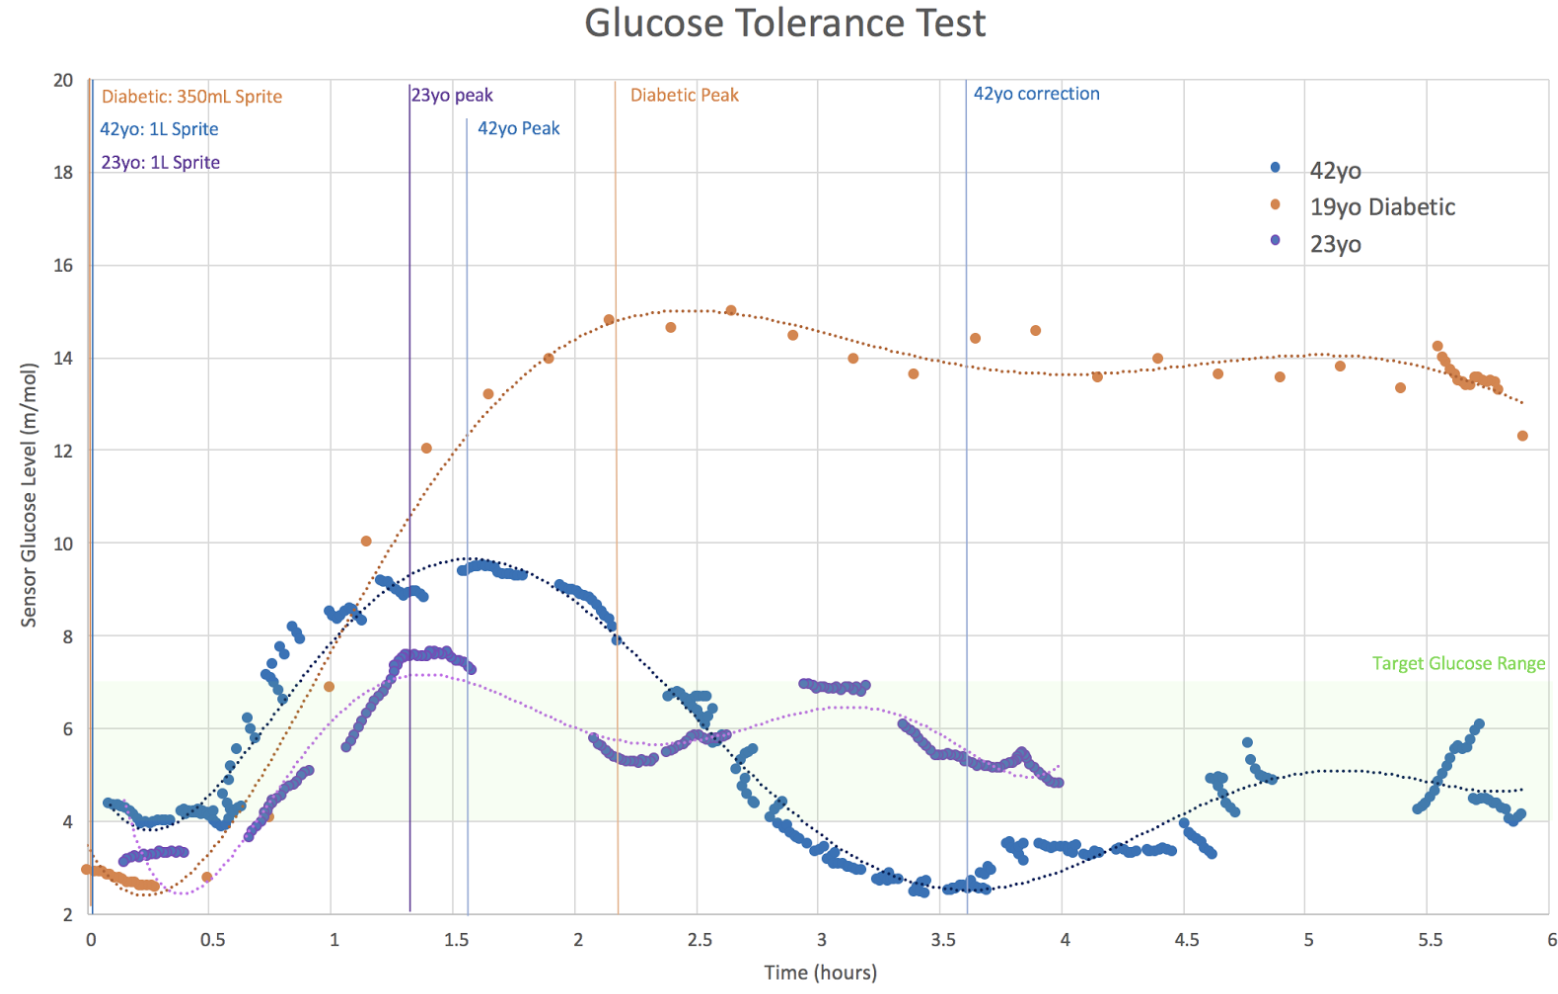
\includegraphics[width=1.0\linewidth]{images/tolerancetest.png}
\caption{Glucose Tolerance Test comparison.}
\label{fig:tolerancetest}
\end{figure}

Our testing, while far from extensive, did give some insight into the glucose response of three people - 19yo female diabetic, 23yo male non-diabetic, and 42yo male non-diabetic. Figure~\ref{fig:tolerancetest} shows the aftermath of a glucose tolerance test (note, the diabetic’s serving size was lowered to avoid health concerns). It’s clear that the younger male has a quicker insulin response to the sugar, peaking at 7.6 mmol/L just 1hr 20 mins after consumption. The older male peaks 15min later at 1hr 35 mins, with a high of 9.5 mmol/L. The post-peak decline is particularly interesting. Although the 42yo peaked later, his glucose response actively turned his blood glucose around and actually pushed him into hypoglycemia for an hour before correcting. The 23yo’s reaction, on the other hand, kicked in earlier and leveled out the high. This is apparent from the first derivative (Figure~\ref{fig:derivatives}), which shows the 23yo’s blood glucose rate of change dropping off sharply. However, although it then decreases somewhat, the drop is comparatively restrained. Interestingly, despite the lack of hypoglycemia, there still appears to be a corrective response. 

\begin{figure}[!htb]
\centering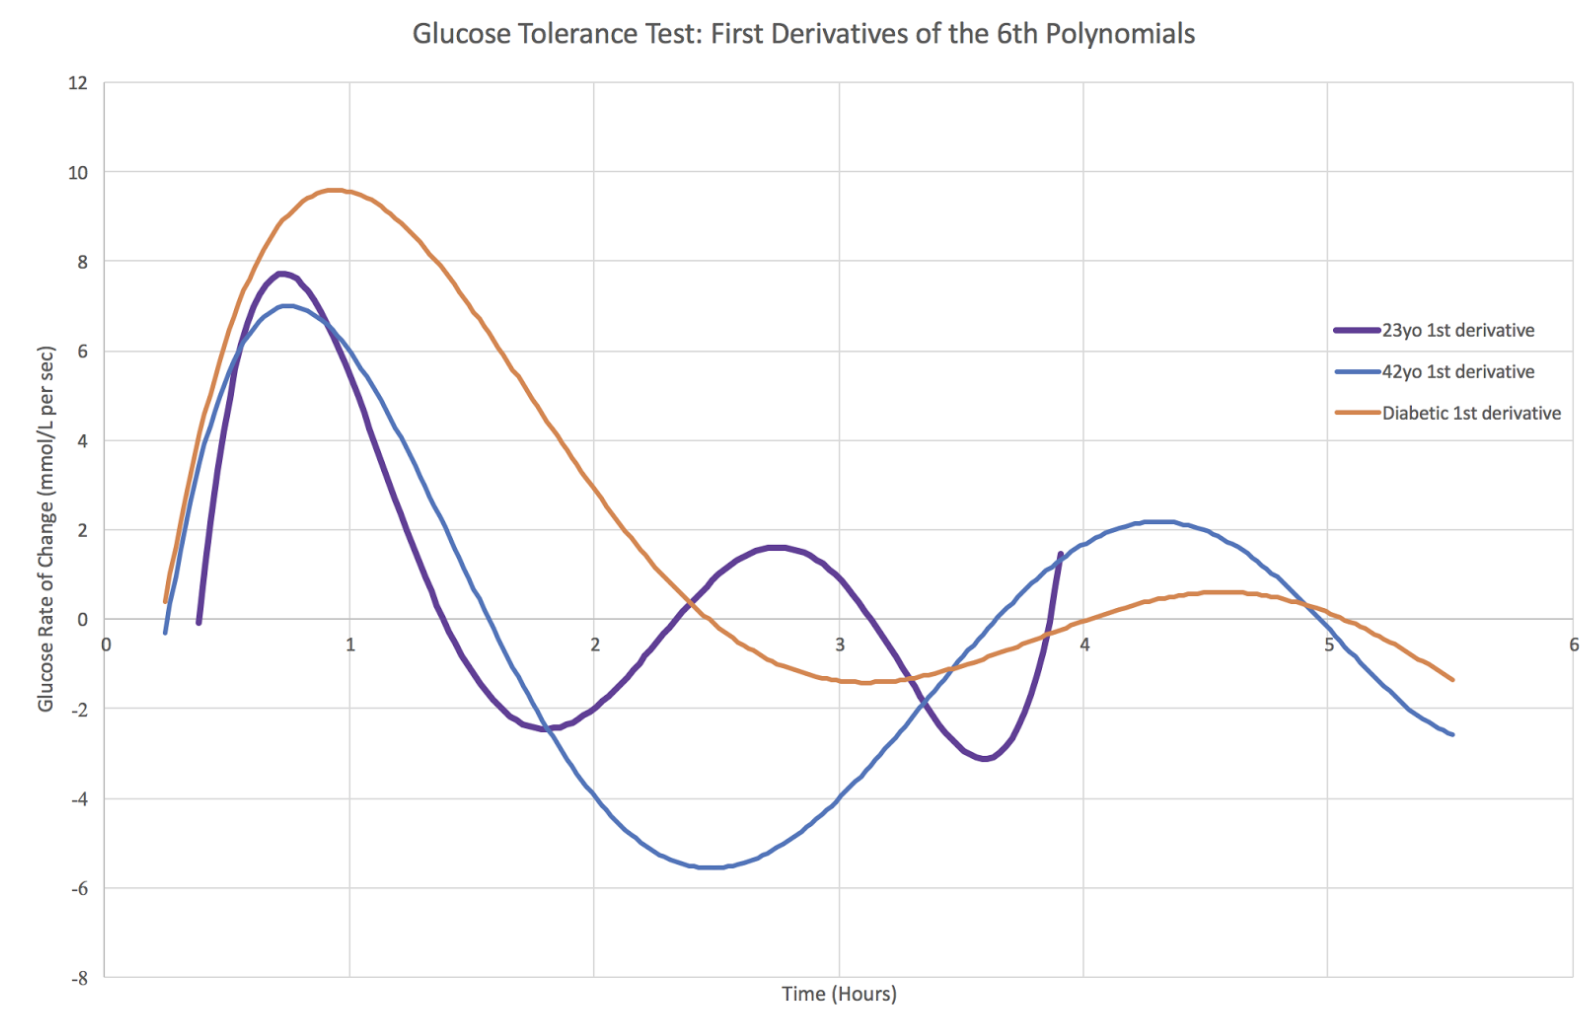
\includegraphics[width=1.0\linewidth]{images/derivatives.png}
\caption{First derivative of the glucose responses (from fitted sixth degree polynomial).}
\label{fig:derivatives}
\end{figure}

In contrast, the diabetic does not appear to have any counter-reaction to the sugar. Her blood glucose continues to rise to 15mmol/L, when it appears to have run through the sugar over two hours past consumption. It then plateaus, although appears to decrease over time. This is understandable, since a diabetic has limited to zero internal glucose regulation, and instead has to rely on insulin (typically both short-term and long-term) to manage levels. Continuous monitoring can also provide an interesting insight into the effectiveness of this management. 

\begin{figure}[!htb]
\centering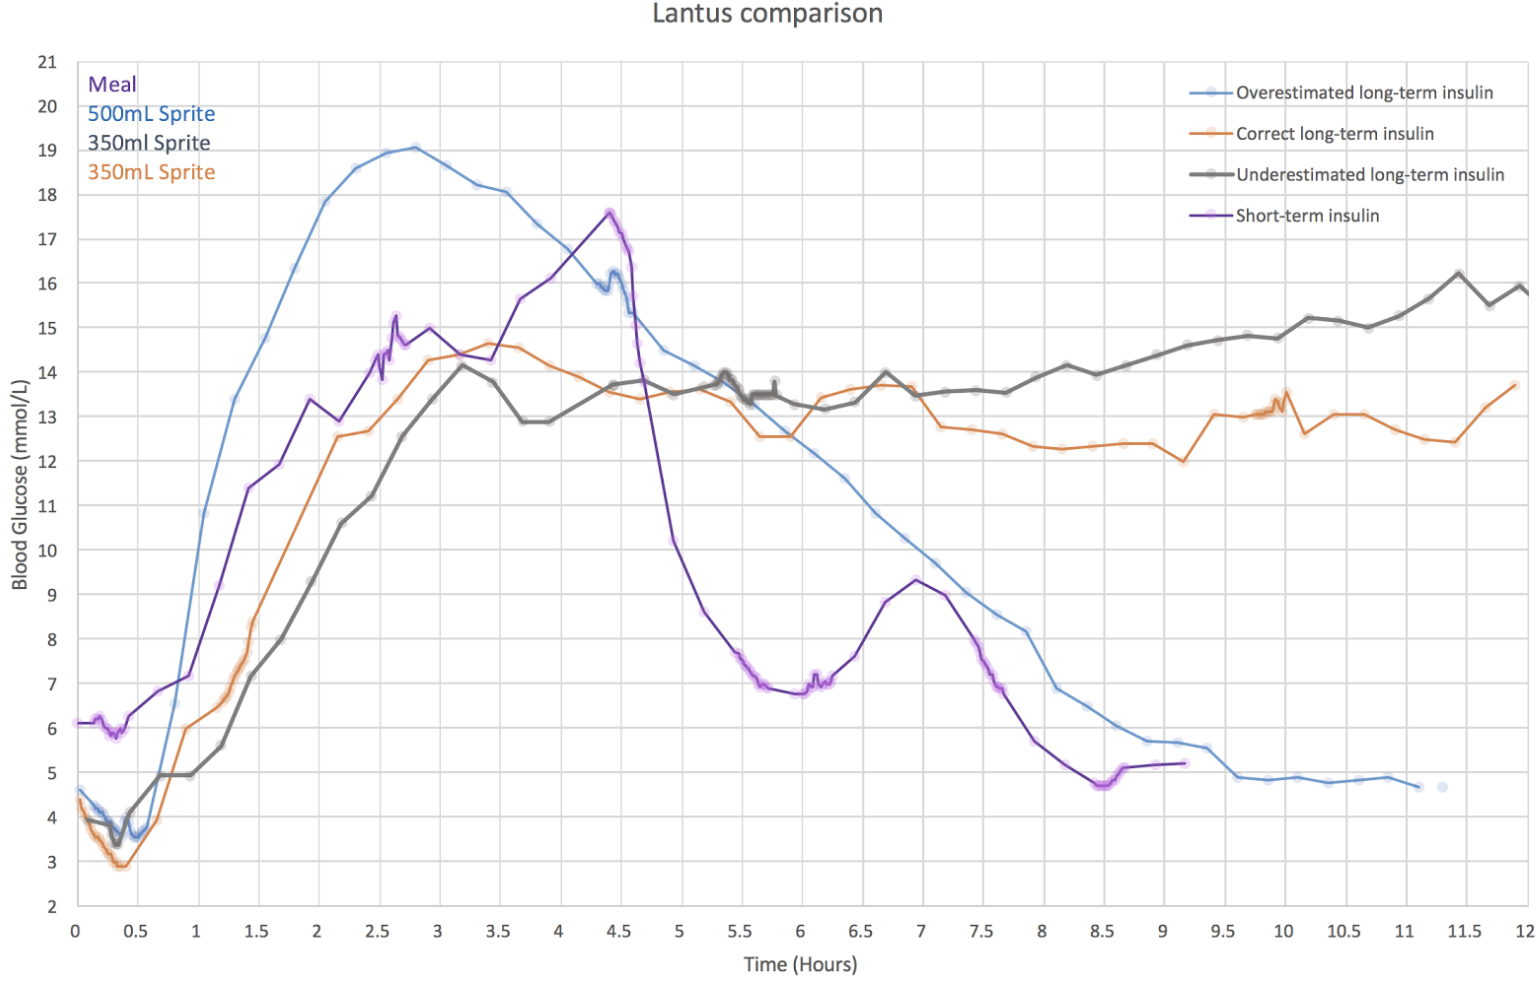
\includegraphics[width=1.0\linewidth]{images/lantuscompare.png}
\caption{Comparison of the effects of different insulin treatments post-food in everyday life.}
\label{fig:lantuscompare}
\end{figure}

Figure~\ref{fig:lantuscompare} shows revealing CGM data from different insulin combinations in the course of everyday life. The appropriateness of long-term insulin, in particular, becomes readily apparent from CGM data, which show whether blood glucose decreases over time without further action, increases, or stays steady as desired. This level of understanding is very difficult to gain from the discrete and limited nature of BGM data, especially as temporary interference (from food, short-term insulin, exercise, etc) can confound any of the few spotchecks. The CGM data is very easy to interpret on this front. This also provides better monitoring of short-term insulin. In Figure~\ref{fig:lantuscompare}, this is given away by the steep post-peak curve. However, it’s surprising how long it took to take noticeable effect - three hours, on the inside. This may, however, be more indicative of eating patterns (spending hours nibbling over dinner instead of rushing it down) than issues with the insulin. This would be an interesting point to further research. 